    \begin{itemize}
        \item Utilizando búsqueda unidimensional.

\begin{table}[H]
\centering
\renewcommand{\arraystretch}{1.2} 
\begin{tabular}{|c|c|c|c|c|c|c|}
\hline
\textbf{Iter$_{total}$} &\textbf{x$_{inicial}$} & \textbf{$x^k$} & \textbf{||$\nabla \mathbf{f(x^k)}$}|| & \textbf{f($\mathbf{x^k}$)} &  \textbf{tiempo} \\
\hline
2  &  (0.24 , 0.85) &( 0.0000,0.0000 ) & 0.00000000 & -1.00000000 & 0.2568 \\
2  &  (0.09 , 0.43) &( 0.0000,0.0000 ) & 0.00000000 & -1.00000000 & 0.1800 \\
2  &  (0.85 , 0.12) &( -0.0000,-0.0000 ) & 0.00000000 & -1.00000000 & 0.1790 \\
2  &  (0.34 , 0.15) &( 0.0000,0.0000 ) & 0.00000000 & -1.00000000 & 0.2443 \\
2  &  (0.9 , 0.26) &( 0.0000,0.0000 ) & 0.00000000 & -1.00000000 & 0.2903 \\
2  &  (0.06 , 0.86) &( 0.0000,0.0000 ) & 0.00000000 & -1.00000000 & 0.2665 \\
2  &  (0.59 , 0.78) &( -0.0000,-0.0000 ) & 0.00000000 & -1.00000000 & 0.1710 \\
1  &  (1.9 , 5.49) &( 1.9000,5.4900 ) & 0.00000000 & -0.00000000 & 0.0000 \\
2  &  (1.29 , 2.26) &( -0.0000,-0.0000 ) & 0.00000000 & -1.00000000 & 0.1530 \\
1  &  (2.4 , 3.38) &( 2.4000,3.3800 ) & 0.00000029 & -0.00000003 & 0.0000 \\
1  &  (3.42 , 3.87) &( 3.4200,3.8700 ) & 0.00000000 & -0.00000000 & 0.0000 \\
2  &  (2.46 , 2.07) &( -0.0000,-0.0000 ) & 0.00000000 & -1.00000000 & 0.1562 \\
1  &  (5.65 , 6.18) &( 5.6500,6.1800 ) & 0.00000000 & -0.00000000 & 0.0000 \\
2  &  (2.46 , 2.18) &( 0.0000,0.0000 ) & 0.00000000 & -1.00000000 & 0.1553 \\
2  &  (1.28 , 1.49) &( -0.0000,-0.0000 ) & 0.00000000 & -1.00000000 & 0.2673 \\
2  &  (1.28 , 2.49) &( -0.0000,-0.0000 ) & 0.00000000 & -1.00000000 & 0.2898 \\
1  &  (3.78 , 2.62) &( 3.7800,2.6200 ) & 0.00000001 & -0.00000000 & 0.0000 \\

\hline
\end{tabular}
\end{table}

\begin{figure}
    \centering
    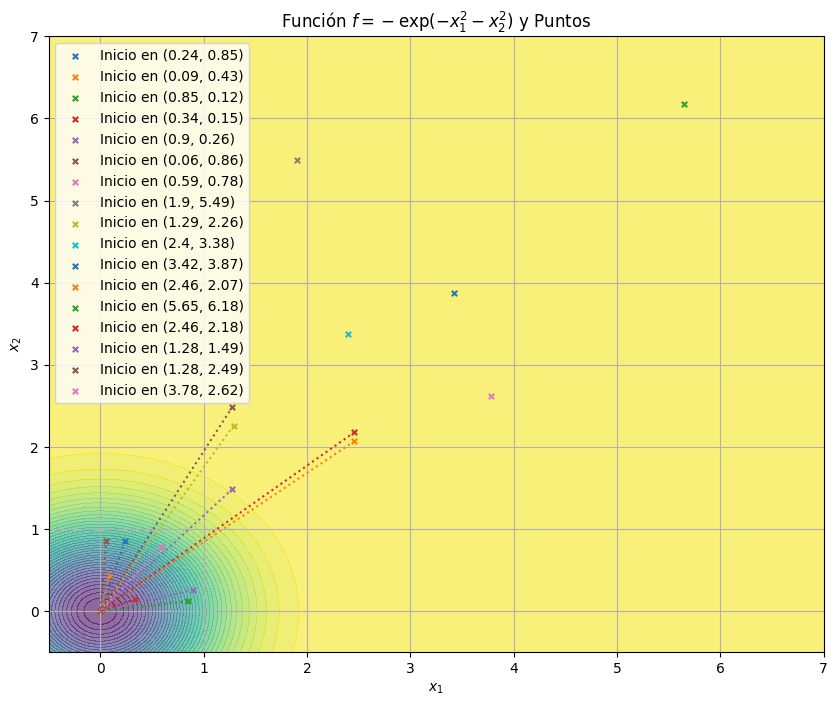
\includegraphics[width=0.73\linewidth]{figuras/PREG4_UNI.png}
    \label{fig:enter-label}
\end{figure}


        \item  Utilizando busqueda de Armijo.
        
\begin{table}[H]
\centering
\renewcommand{\arraystretch}{1.2}
\begin{tabular}{|c|c|c|c|c|c|c|}
\hline
\textbf{It$_{total}$} & \textbf{Arm$_{total}$} & \textbf{$x_{inicial}$} & \textbf{$\mathbf{x^k}$} & \textbf{|| $\nabla$f($\mathbf{x^k}$) ||} & \textbf{f($\mathbf{x^k}$)} & \textbf{tiempo} \\
\hline
3  & 5 &  (0.24 , 0.85) &( 0.0000,0.0000 ) & 0.00000000 & -1.00000000 & 0.0530 \\
3  & 6 &  (0.09 , 0.43) &( 0.0000,0.0000 ) & 0.00000000 & -1.00000000 & 0.0626 \\
3  & 5 &  (0.85 , 0.12) &( 0.0000,0.0000 ) & 0.00000000 & -1.00000000 & 0.0360 \\
3  & 6 &  (0.34 , 0.15) &( 0.0000,0.0000 ) & 0.00000000 & -1.00000000 & 0.0450 \\
3  & 5 &  (0.9 , 0.26) &( 0.0000,0.0000 ) & 0.00000012 & -1.00000000 & 0.0343 \\
3  & 5 &  (0.06 , 0.86) &( 0.0000,0.0000 ) & 0.00000000 & -1.00000000 & 0.0320 \\
5  & 10 &  (0.59 , 0.78) &( 0.0000,0.0000 ) & 0.00000000 & -1.00000000 & 0.0382 \\
0  & 0 &  (1.9 , 5.49) &( 1.9000,5.4900 ) & 0.00000000 & -0.00000000 & 0.0000 \\
45  & 47 &  (1.29 , 2.26) &( -0.0000,-0.0000 ) & 0.00000007 & -1.00000000 & 0.3310 \\
0  & 0 &  (2.4 , 3.38) &( 2.4000,3.3800 ) & 0.00000029 & -0.00000003 & 0.0000 \\
0  & 0 &  (3.42 , 3.87) &( 3.4200,3.8700 ) & 0.00000000 & -0.00000000 & 0.0000 \\
847  & 850 &  (2.46 , 2.07) &( 0.0000,0.0000 ) & 0.00000000 & -1.00000000 & 5.3212 \\
0  & 0 &  (5.65 , 6.18) &( 5.6500,6.1800 ) & 0.00000000 & -0.00000000 & 0.0000 \\
1281  & 1284 &  (2.46 , 2.18) &( 0.0000,0.0000 ) & 0.00000000 & -1.00000000 & 7.3310 \\
9  & 12 &  (1.28 , 1.49) &( 0.0000,0.0000 ) & 0.00000000 & -1.00000000 & 0.0969 \\
102  & 105 &  (1.28 , 2.49) &( 0.0000,0.0000 ) & 0.00000007 & -1.00000000 & 0.5136 \\
0  & 0 &  (3.78 , 2.62) &( 3.7800,2.6200 ) & 0.00000001 & -0.00000000 & 0.0000 \\
\hline
\end{tabular}
\end{table}
Para el gráfico se encuentra lo siguiente:

\begin{itemize}
    \item La trayectoria 8 está vacía.
    \item La trayectoria 10 está vacía.
    \item La trayectoria 11 está vacía.
    \item La trayectoria 13 está vacía.
    \item La trayectoria 17 está vacía.
\end{itemize}



\begin{figure}
    \centering
    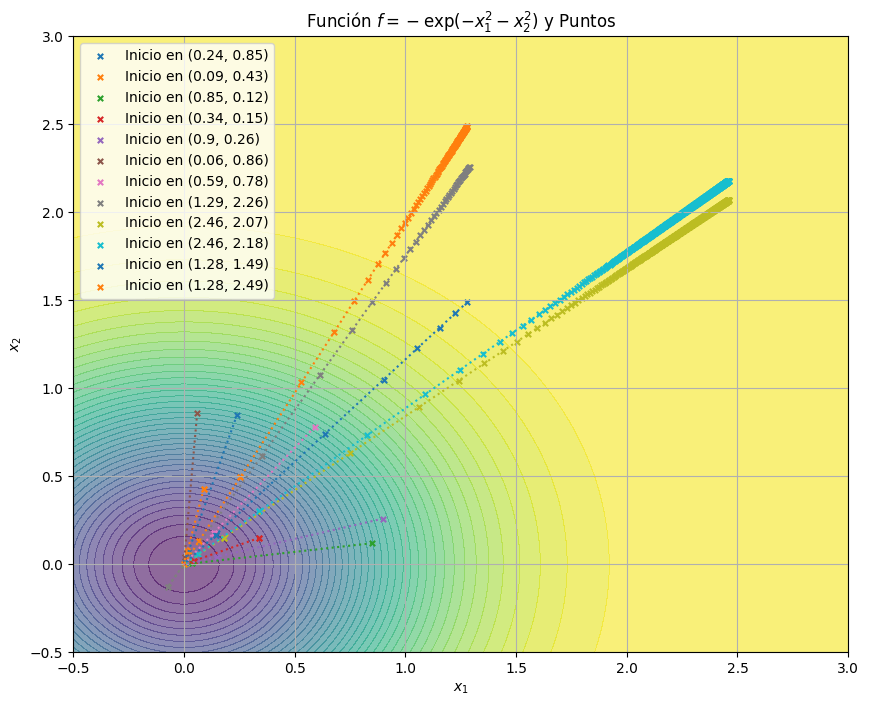
\includegraphics[width=0.75\linewidth]{figuras/PREG4_ARMIJO.png}
    \label{fig:enter-label}
\end{figure}